\normaltrue \difficilefalse \tdifficilefalse
\correctionfalse

%\UPSTIidClasse{11} % 11 sup, 12 spé
%\newcommand{\UPSTIidClasse}{12}
% ATS 2019
\exer{Le banc balafre $\star$ \label{SYS:01:50}}
\setcounter{question}{0}\marginnote{\xpComp{SYS}{01}}
\index{Compétence SYS-01}
\index{Le Banc Balafre}
\index{Caractériser un constituant de la chaîne d’information.}
\index{Capteurs}
\ifcorrection
\else
\marginnote{\textbf{Pas de corrigé pour cet exercice.}}
\fi

\ifprof
\else


Entre autres contrôles de la chaîne d’acquisition, le superviseur vérifie que la mesure des efforts se fait correctement : au niveau des actionneurs piézoélectriques et au niveau du joint testé. Les capteurs de force utilisés sur le système sont analogiques. Afin de simplifier le traitement et l’interprétation de ces forces, on utilise un amplificateur de charges à plusieurs canaux (voir figure \ref{fig_50_01}).


\begin{marginfigure}
\centering
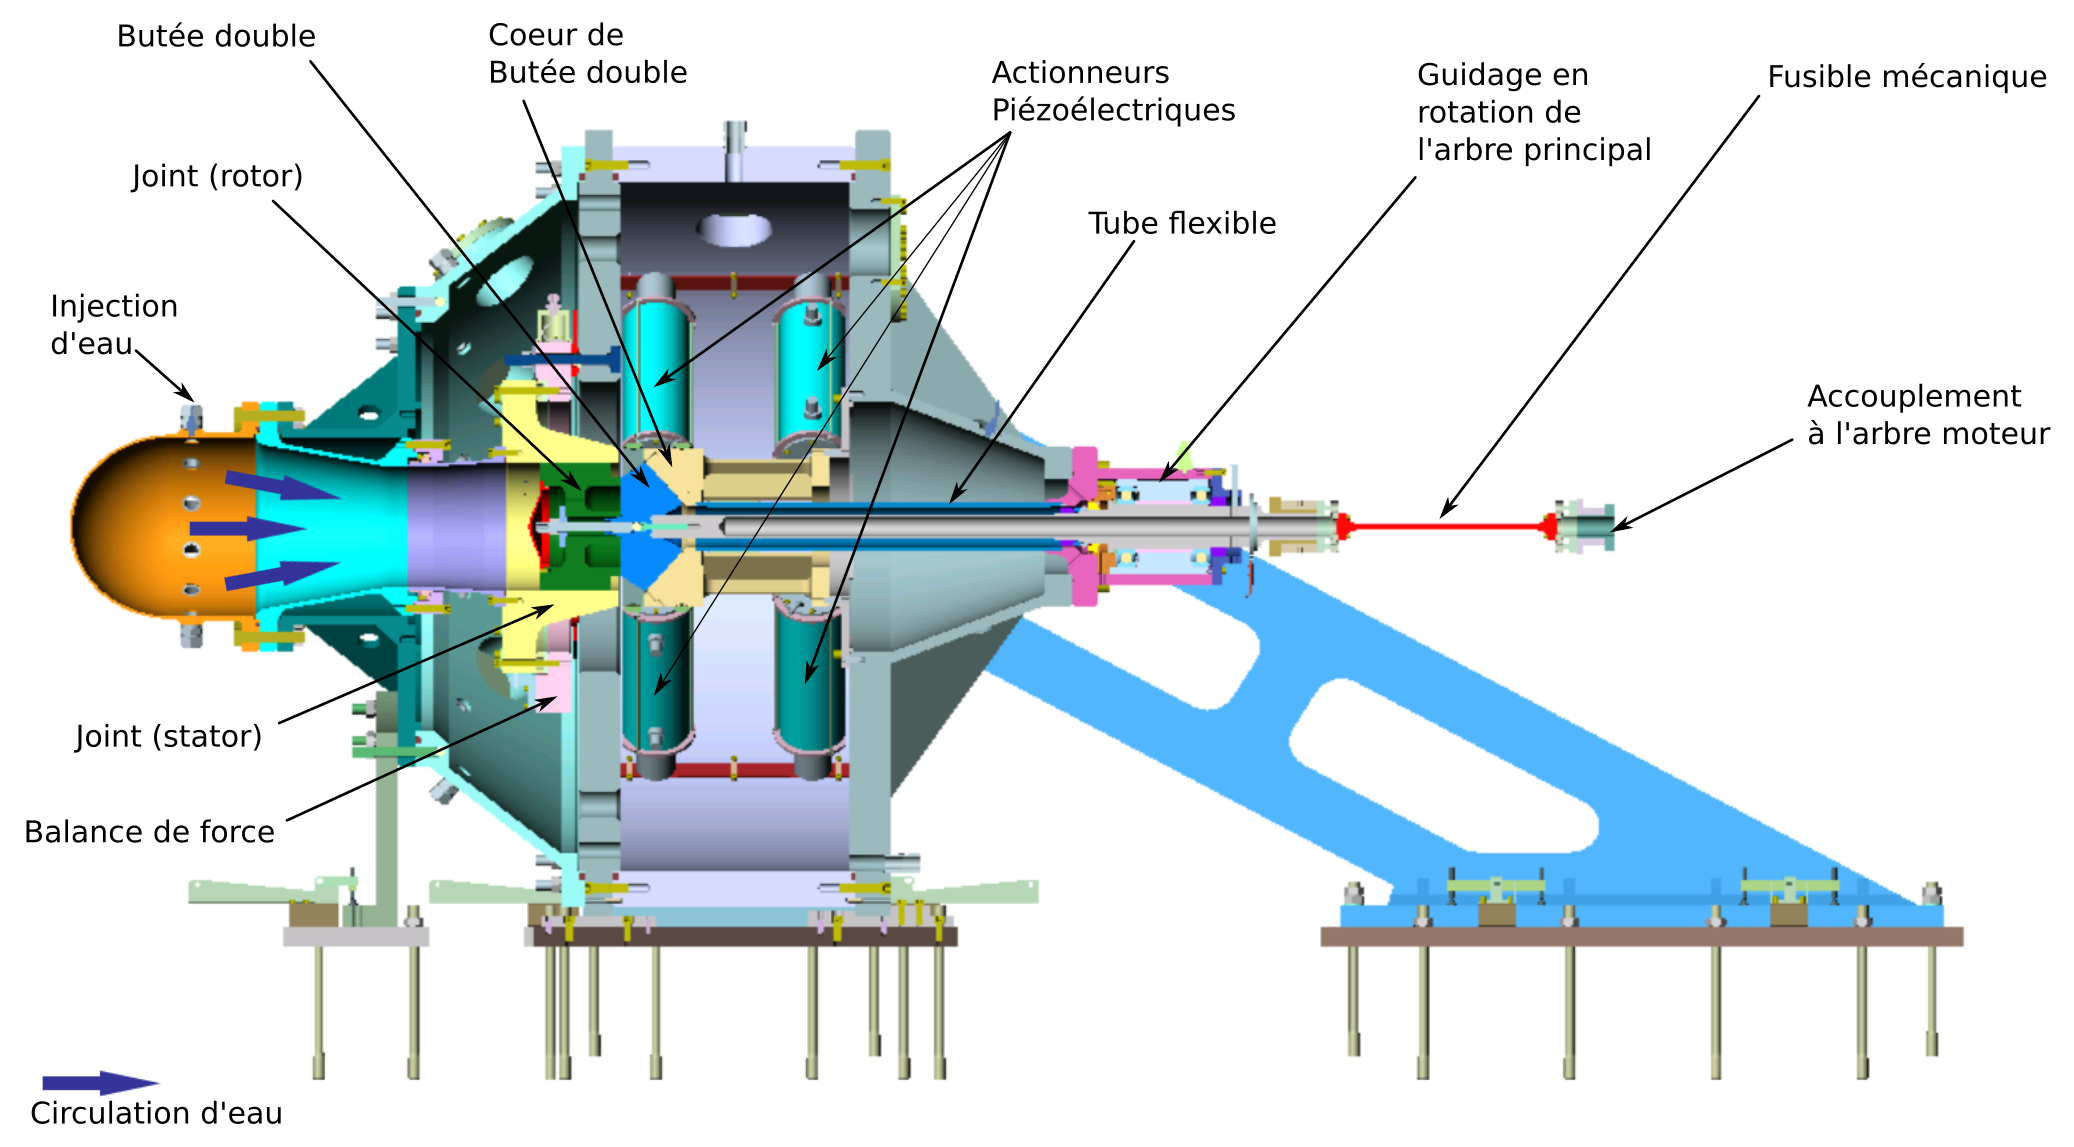
\includegraphics[width=\linewidth]{fig_50_01}
\caption{Amplificateur de charge à plusieurs canaux KISTLER. \label{fig_50_01}}
\end{marginfigure}



Cet amplificateur possède deux options qui sont utilisées sur le banc Balafre :
\begin{itemize}
\item l’amplificateur de sommation pour le calcul analogique des forces et moments résultants
;
\item un convertisseur Analogique/Numérique pour faire le traitement des données (algorithme
de contrôle).
\end{itemize}
Dans l’algorithme de contrôle, la valeur d’effort de chaque actionneur est comparée à
la valeur théorique de la consigne effectuée pour le contrôle. Si un écart trop grand est
constaté, l’algorithme de contrôle émet un signal d’erreur (Controle=2). Pour cette mesure,
on considère qu’une résolution inférieure à  \SI{10}{N} est nécessaire.
La conversion analogique/numérique se fait ici sur 12 bits. La mesure de l’effort se fait
sur la plage de $-20$ à \SI{20}{kN}. Les données techniques utiles sont rassemblées sur la figure
\ref{fig_50_02}.

\begin{marginfigure}
\centering
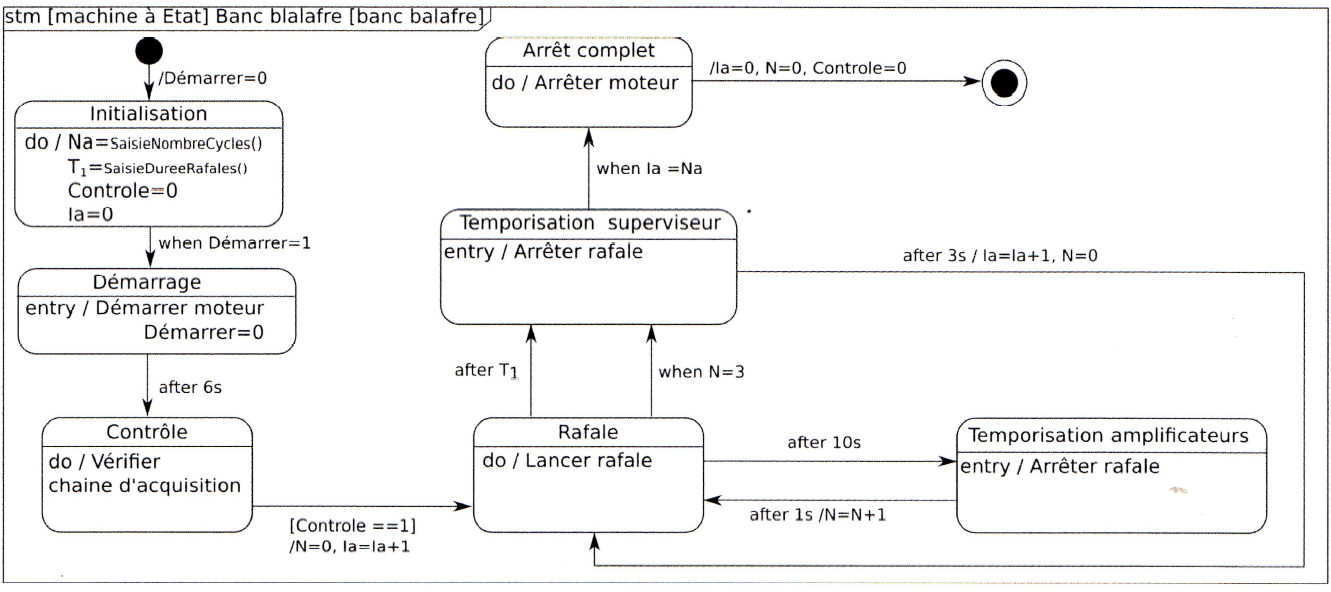
\includegraphics[width=.7\linewidth]{fig_50_03}
\caption{Capteur de force KISTLER 9167A. \label{fig_50_03}}
\end{marginfigure}

Le capteur de force (voir figure \ref{fig_50_03}) utilisé est un capteur KISTLER 9167A, permettant
de mesurer des efforts dans trois directions. Pour la mesure de l’effort développé par
les actionneurs, seule la direction Z est utilisée, et la sensibilité du capteur dans cette
direction est \SI{4,2}{pC.N^{-1}}.
Le synoptique de la figure \ref{fig_50_04} présente la structure interne de l’amplificateur de charge.

\begin{figure}[H]
\centering
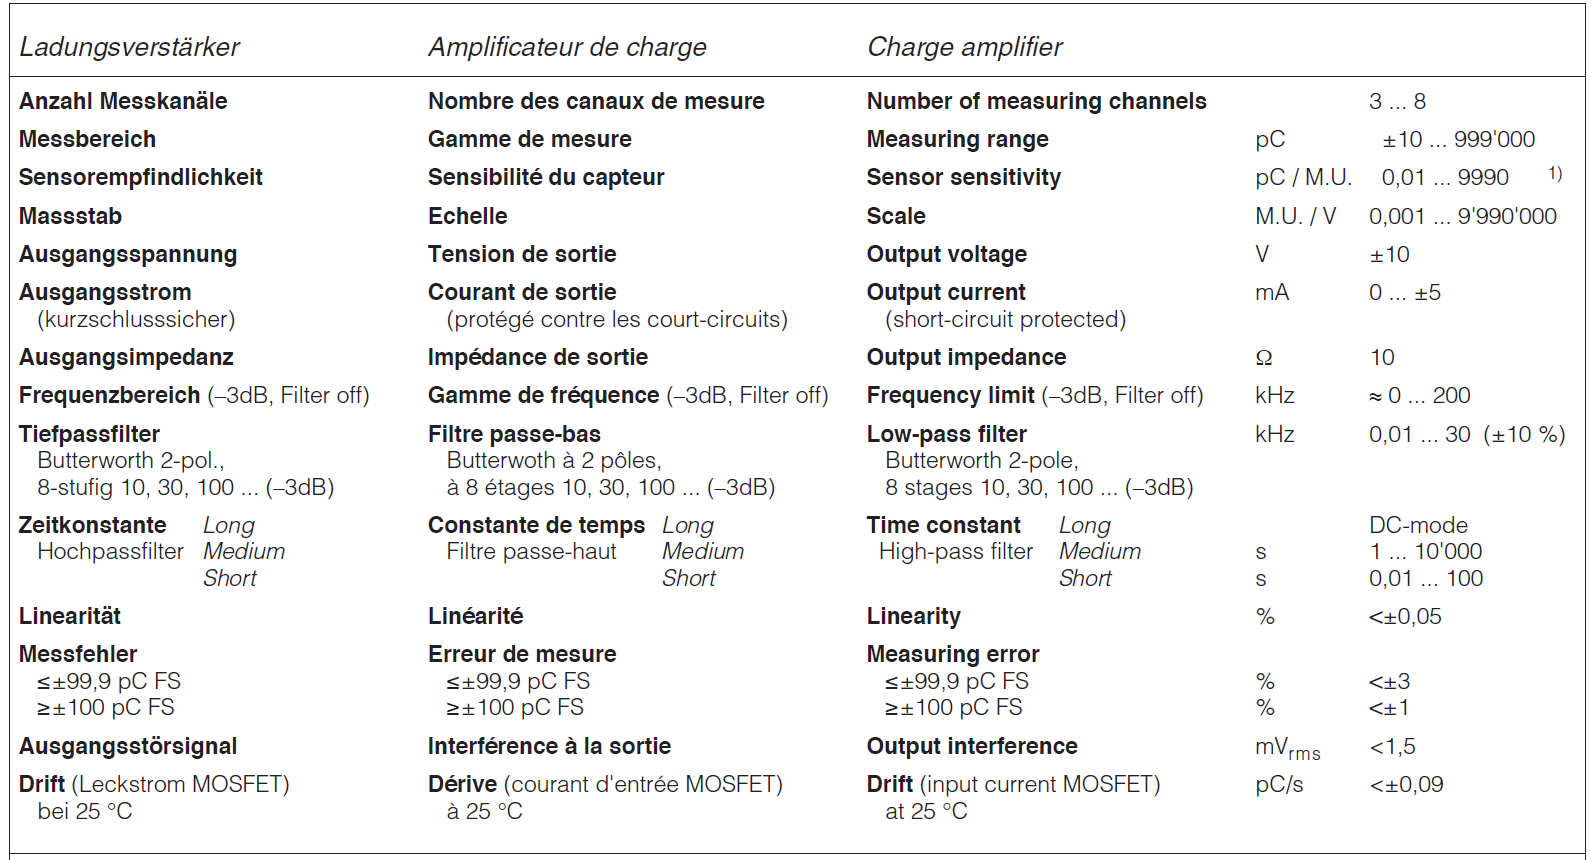
\includegraphics[width=\linewidth]{fig_50_02}
\caption{Amplificateur de charge à plusieurs canaux KISTLER. \label{fig_50_02}}
\end{figure}



\begin{figure}[H]
\centering
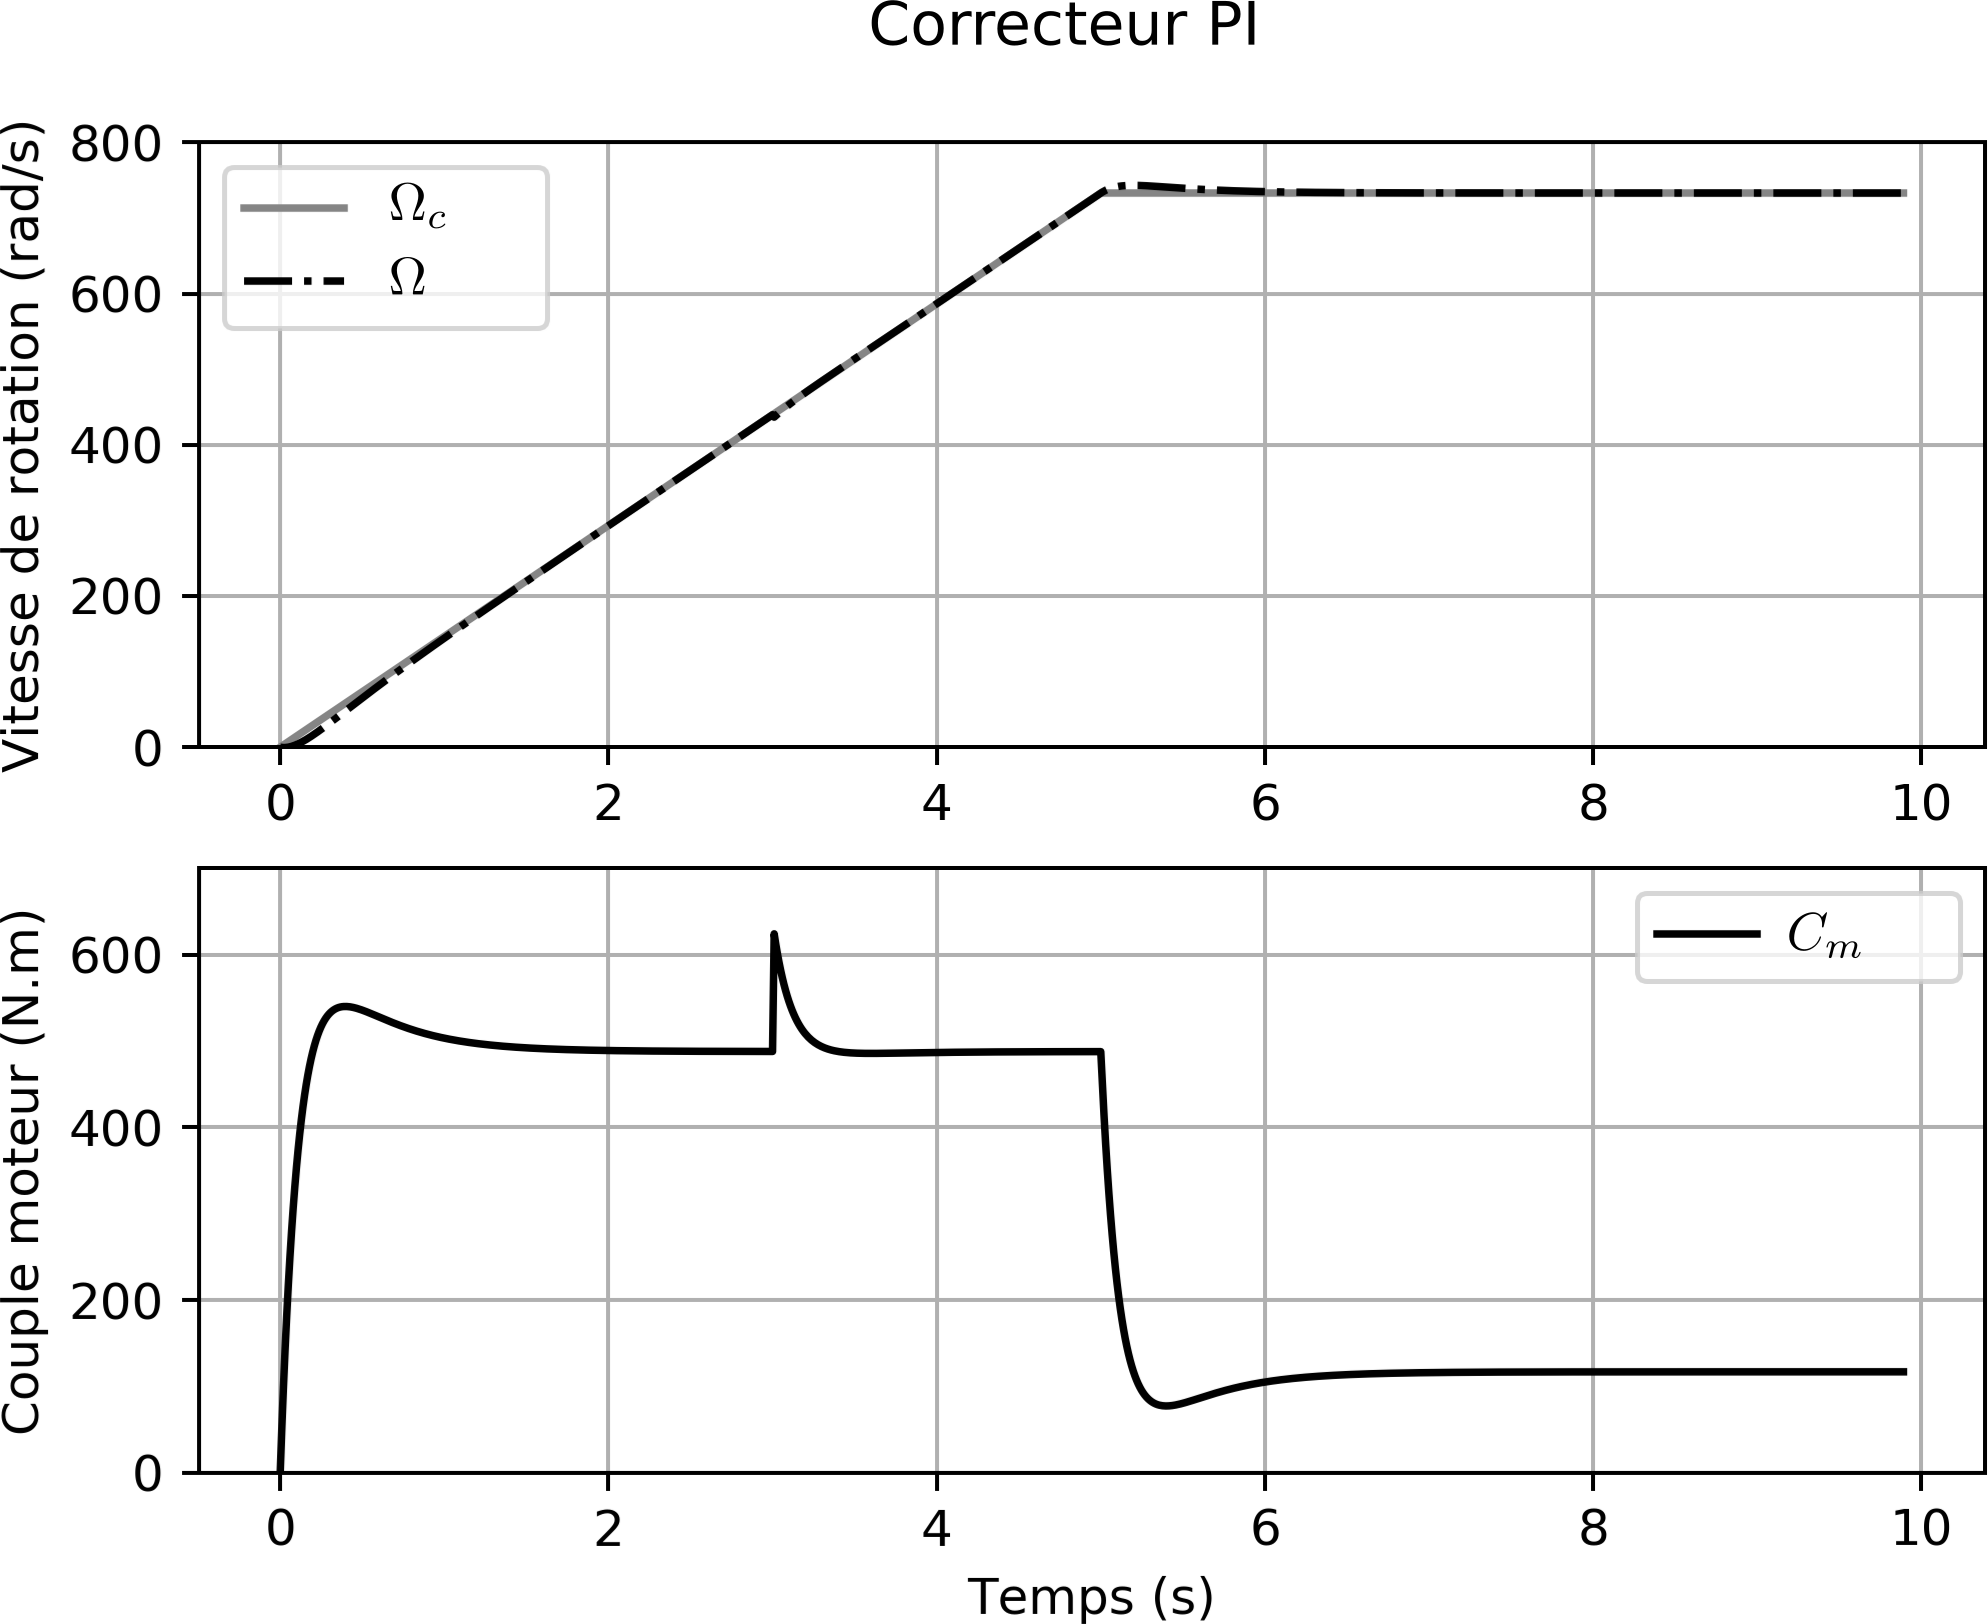
\includegraphics[width=\linewidth]{fig_50_04}
\caption{Synoptique de la structure interne de l’amplificateur de charge. \label{fig_50_04}}
\end{figure}
\fi

\question{Sur le synoptique de la figure \ref{fig_50_04}, on peut lire « Analog to Digital Converter Multiplexed ». Que signifie le terme multiplexé utilisé ici ?}
\ifprof
\else
\fi

\question{Compte tenu de la sensibilité du capteur et de l’étendue des valeurs à
mesurer, déterminer la gamme de mesure à régler sur l’amplificateur de charge.}
\ifprof
\else
\fi

\question{En utilisant la documentation technique de l’amplificateur de charge,
déterminer la plage de variation de la tension de sortie de l’amplificateur. En déduire le
quantum de la conversion analogique numérique, puis la résolution de la mesure. Conclure
vis-à-vis de la résolution demandée.}
\ifprof
\else
\fi




\ifprof
\else
\begin{flushright}
\footnotesize{Corrigé  voir \ref{SYS:01:50}.}
\end{flushright}%
\fi